% -----------------------------------------------------------------------------
% Metodologia
% -----------------------------------------------------------------------------

\chapter{Metodologia}
\label{chap:metodologia}
\section{Disponibilidade dos recursos deste trabalho}
Todos os componentes definidos nesse trabalho estarão contidos em um ou mais repositórios públicos, garantindo a livre apreciação da comunidade não só científica, mas a todos os interessados na contribuição ou utilização sob a licença pública geral GNU versão 3 \cite{foss2022}.

\section{Especificação dos nós integrantes do  \emph{cluster} de baixo custo}

A formação do  \emph{cluster} será de máquinas virtuais (VMs) e/ou físicas que possuem custo e capacidade computacionais mais baixos, com configurações comumente encontradas em computadores do tipo desktops, como os utilizados em residências, escritórios e laboratórios de informática genéricos.

A primeira versão dessa solução será realizada de maneira simulada, utilizando ambiente virtualizado com VMs que, por sua vez, serão provisionadas em \emph{hypervisors} do tipo 2 \cite{comer_cloud_2021} (\emph{hosted} \emph{hypervisor}), para garantir a simplicidade da implementação da primeira fase (TCC I) e validar o conceito de provisionamento, configuração e \emph{deploy} de aplicações testes e laboratório das ferramentas de monitoramento que serão utilizadas, a serem descritas na sessão \ref{cap:monitor}. 

A versão final do projeto (ambas constarão no TCC II) visa o provisionamento do  \emph{cluster} nos ambientes de teste configurados como descrito na sessão \ref{sec:abordagem}, sendo que algumas premissas serão utilizadas, como o uso de mesmo sistema operacional e versão em cada um desses computadores, garantindo a redução de configuração necessária para a implementação. Outra premissa utilizada para esse estudo será a utilização de uma rede comum aos computadores. 

O aproveitamento de computadores comuns já existentes e subutilizados, seja por uso abaixo de sua capacidade ou ainda intervalos de ociosidade, qualifica o baixo custo da formação do  \emph{cluster} em questão, apresentando CAPEX (capital expenditure),  ou investimento inicial mínimo, se não zero, necessitando da interdisciplinaridade sugerida e defendida dentro das instituições para as quais esse trabalho intenta apresentar uma alternativa.

\section{Plataforma de orquestração de carga de trabalho}

A plataforma de  \emph{cluster} e orquestração de cargas de trabalho utilizadas nesse trabalho será o Kubernetes. A arquitetura de implementação do  \emph{cluster} será de \emph{multi-master} com etcd \cite{etcd2022} (controlador de logs, e estado do  \emph{cluster}) atachado \cite{kubernetes2022}, ou rodando nos mesmos computadores masters do  \emph{cluster}. 
Essa arquitetura (figura \ref{fig:kubeadmha} recomendada garante a alta disponibilidade do  \emph{cluster}, importante para que não haja interrupções inesperadas durante a orquestração das cargas de trabalho (execução, disponibilidade e garantia de estado desejado). Apenas não garantindo uma recuperação rápida de quedas dos servidores dos nós (computador/servidor integrante do \emph{cluster}) mestres, significando a perda de todos os estados e, com isso, havendo a necessidade de reconfiguração do  \emph{cluster}. Porém considerando os recursos limitados, na justificativa desse projeto, a alta disponibilidade de estado, significaria na obrigatoriedade do mesmo número de computadores disponibilizados para etcd e masters para controle dos estados.


\begin{figure}[!ht]
    \centering
    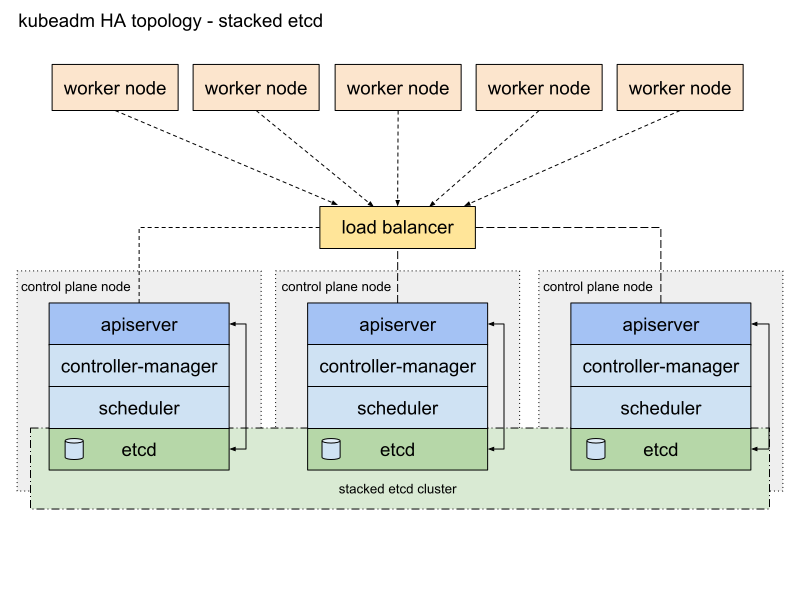
\includegraphics[width=0.8\textwidth]{04-figuras/kubeadm-ha-topology-stacked-etcd.png}
    \caption{Kubernetes Arquitetura de alta disponibilidade (Fonte: The Linux Foundation\textregistered, 2021)}
    \label{fig:kubeadmha}
\end{figure}


Toda a implementação da solução e os componentes relacionados serão conteinerizados, possibilitando  sua orquestração pelo  \emph{cluster} de Kubernetes\textregistered. Apenas as configurações dos  \emph{cluster}s em si e seu provisionamento não estarão conteinerizados. Esses serão disponibilizados em outro repositório específico. 
Para ciclo de vida da aplicação e configurações gerais da solução será utilizada uma estratégia de organização de código em monorepo, sendo essa estratégia a utilização de um repositório único para acompanhamento e desenvolvimento de todos os componentes de software e configurações. O que facilita a visualização, centralização, sincronização e padronização como benefícios primários. conforme citado na literatura, reforçando a adoção dessa estratégia \cite{brito_monorepos_2018}.


\section{Configuração e provisionamento do  \emph{cluster}}
Para provisionamento do \emph{cluster} será utilizado Ansible\textregistered, da empresa RedHat\textregistered que é  um sistema de gerenciamento de configuração (CMS). Sua adoção se deu pela característica minimalista de configuração inicial, facilidade de uso e uma característica fundamental que diminui o \emph{overhead} de operação necessária para sua utilização, não possuir agente instalado no inventário de máquinas gerenciadas. 

O principal ganho na utilização de CMS é a manutenção e replicabilidade de uma determinada configuração e, no caso do Ansible, não há necessidade de configuração prévia ou instalação de nenhum binário específico para sua utilização, reduzindo assim a complexidade de sua adoção.

A configuração inicial é realizada pela disponibilidade de acesso via rede, python na máquina a ter sua configuração gerenciada (asset, ou recurso) e por meio de alguns tipos de autenticação (kerberos, WinRM, SSH etc), sendo no caso utilizado o protocolo SSH \cite{noauthor_rfc4254_nodate} por chaves assimétricas, o que garante um nível aceitável de segurança, especialmente quando é possível escolher os algoritmos de criptografia e suas possíveis variações como RSA e ED25519.

\section{Análise de dados}

O banco de dados “Vendas de Medicamentos Controlados e Antimicrobianos - Medicamentos Industrializados”, disponibilizado pelo governo brasileiro (via portal dados.gov.b), será utilizado nesse trabalho. Os anos correspondentes dos dados são no período entre 2014 e 2021 e o banco possui mais de 70 GB  e mais de 530 milhões de linhas, sendo portanto suficiente para ser utilizado como carga de trabalho ao se calcular uma regressão linear para consumo do medicamento de azitromicina.
Como caso base para comparação e teste do modelo proposto, em termos de tempo para processamento da análise proposta acima, será utilizado um único computador (desktop) com capacidade equivalente a 8 computadores de menor capacidade (1vCPU e 2GB De RAM) designados com nós do  \emph{cluster}, portanto contendo recursos de  8 vCPUs e 16GB de RAM. 

\section{Monitoramento}
\label{cap:monitor}

Serão utilizados para monitoramento de execução das cargas de trabalho o Prometheus\textregistered  e para visualização dos dados Grafana\textregistered, ambos sendo configurados a partir do provisionamento do  \emph{cluster}, ainda com a ferramenta proposta inicialmente Ansible\textregistered. Dessa forma, será possível avaliar parâmetros de taxa de lotação das máquinas base, pelo parâmetro de processador e memória, operações de leitura e escrita no disco e também tráfego de rede. Por meio dessas ferramentas será possível, ainda, avaliar dados de tempo de execução de cargas de trabalho em ambos os ambientes propostos e, assim, poder compará-los quanto a eficiência de uso de hardware.

\section{Comparação entre tipos de virtualização}

A arquitetura do tipo x86 foi o tipo mais comum de arquitetura de computadores e boa parte da tecnologia de virtualização inicialmente foi desenvolvida nessa arquitetura \cite{fayyad_benchmarking_2013}. Nesse contexto, será também utilizado na construção desse trabalho virtualizações com guest e host OS em x86, para garantir que outros estudos possam ser relacionados com os resultados obtidos por esse trabalho.
Como descrito anteriormente, serão utilizadas maquinas virtuais com 2GB de RAM e  \emph{containers} com limitações de mesmo tamanho para a realização de configuração do  \emph{cluster} nesses ambientes, e a partir destes, a execução dos workloads.

O tipo de teste de aplicação será um macrobenchmark (system level benchmark) \cite{huge2008,scheepers2014virtualization} comparando parâmetros de uso de CPU, memória e tempo de execução da carga de trabalho proposta na sessão \ref{cap:monitor} deste trabalho. Os parâmetros serão avaliados tanto na máquina de suporte a virtualização, como também nas máquinas virtuais e  \emph{containers}, bem como o tempo de provisionamento do  \emph{container} da carga de trabalho, tempo de execução e quantidades de falhas.

Esse método USE (Usage, Saturation and Errors) \cite{greg2022} será utilizado para extrair e apresentar métricas e avaliar possíveis problemas. Destaca-se que esse não é o foco do trabalho, mas captura de forma adequada os parâmetros de hardware citados acima.

O controle de tempo será por meio de ferramentas de APM (Application Performance Management) associadas à aplicação da carga de trabalho. Dessa forma, garante-se a avaliação de qualidade e possíveis problemas, além de tempos de execução, dentre outros possíveis problemas e métricas de performance da aplicação \cite{tang2021systematical}.


\section{Cronograma}
A primeira parte do Trabalho de Conclusão de Curso consiste em um estudo dos métodos de virtualização, plataformas elegidas como possíveis soluções e a composição de arquitetura da plataforma de orquestração das cargas de trabalho. O TCCI também serviu para a elaboração de um modelo inicial e também para definição de uma arquitetura de referência a ser refinada no TCC II junto aos demais diagramas do sistema.

A solução proposta para realizar tanto a orquestração, como também a comparação das cargas de trabalho serão validadas durante a execução do TCC II.
Na Figura \ref{fig:cronograma} é apresentado o cronograma completo do projeto.

\begin{landscape}
\begin{figure}[!ht]
    \centering
    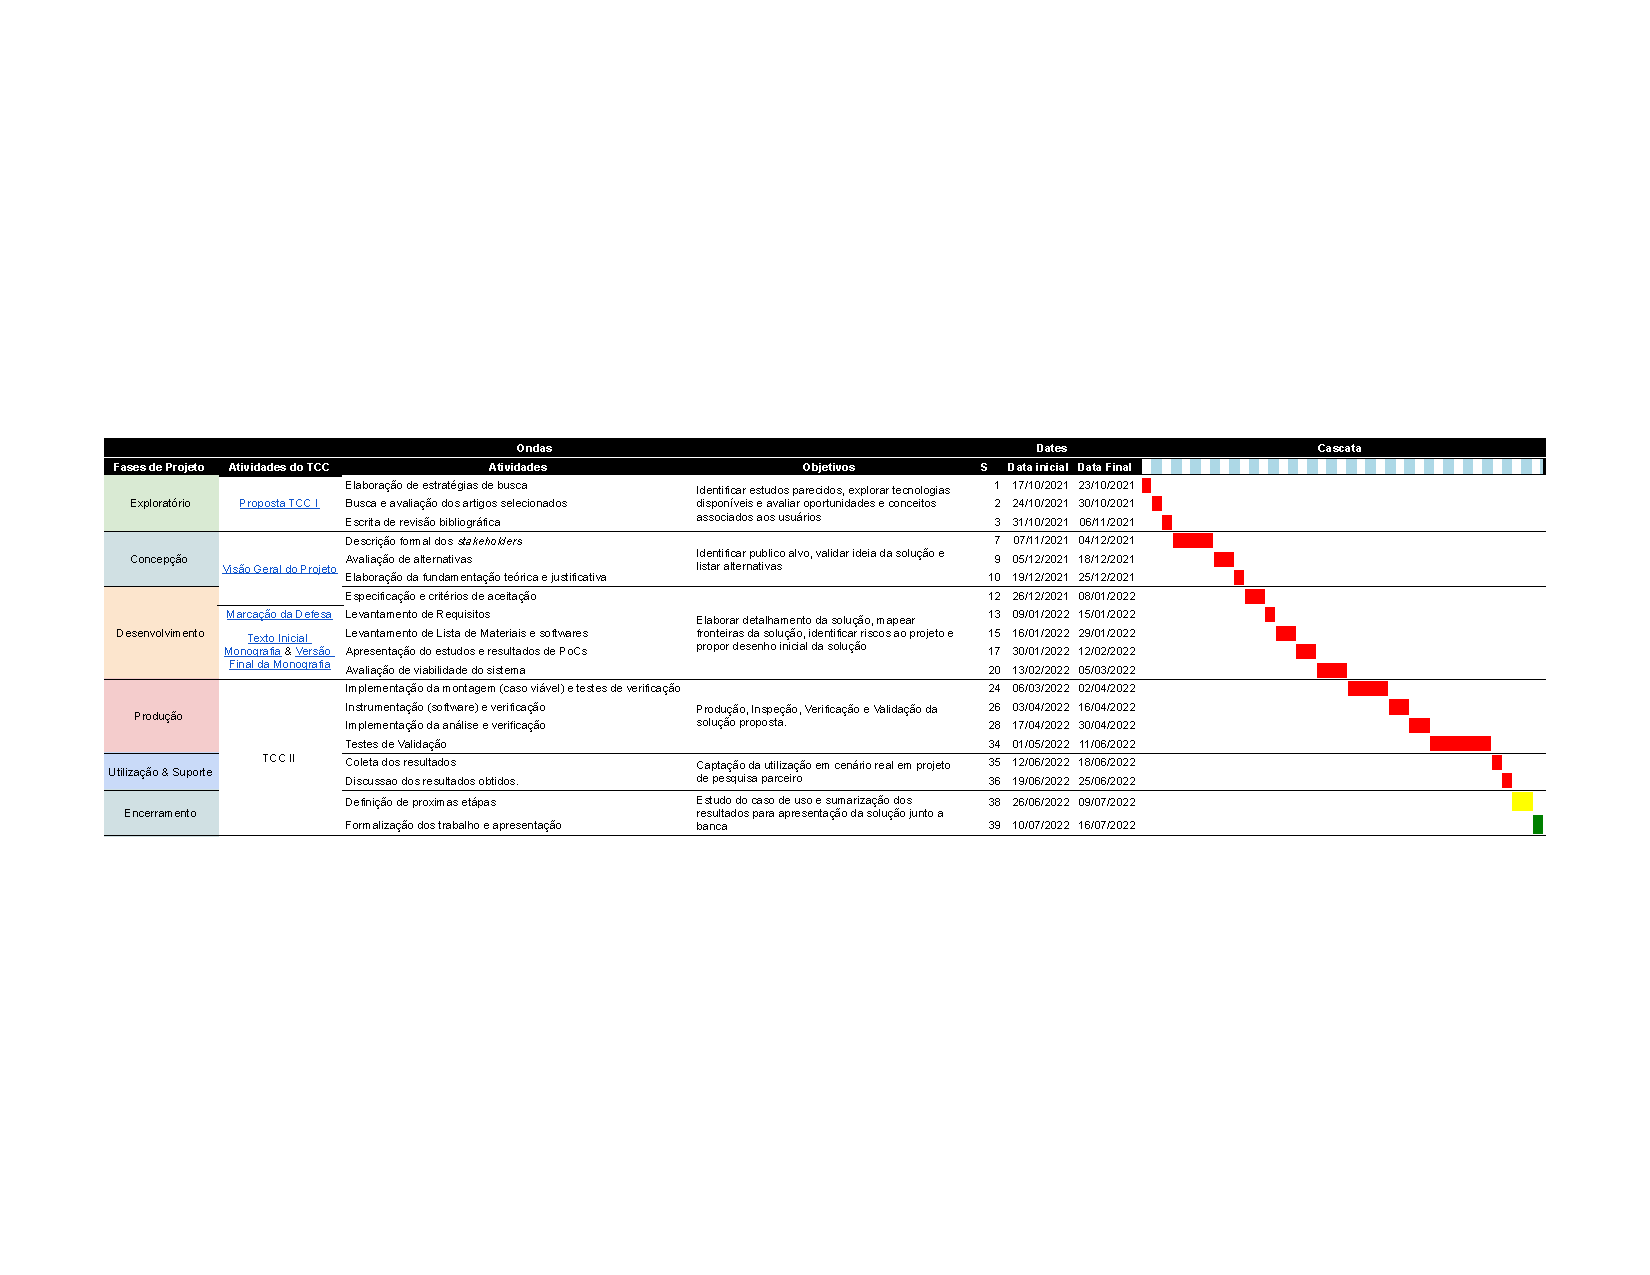
\includegraphics[width=\linewidth]{04-figuras/TCC cronograma - Sheet1.pdf}
    \caption{Cronograma geral do trabalho}
    \label{fig:cronograma}
\end{figure}
\end{landscape}